\documentclass[tikz,border=12pt]{standalone}
\usetikzlibrary{arrows.meta, positioning, calc, decorations.pathreplacing}
\usepackage{amsmath}
\usepackage{amssymb}

\begin{document}
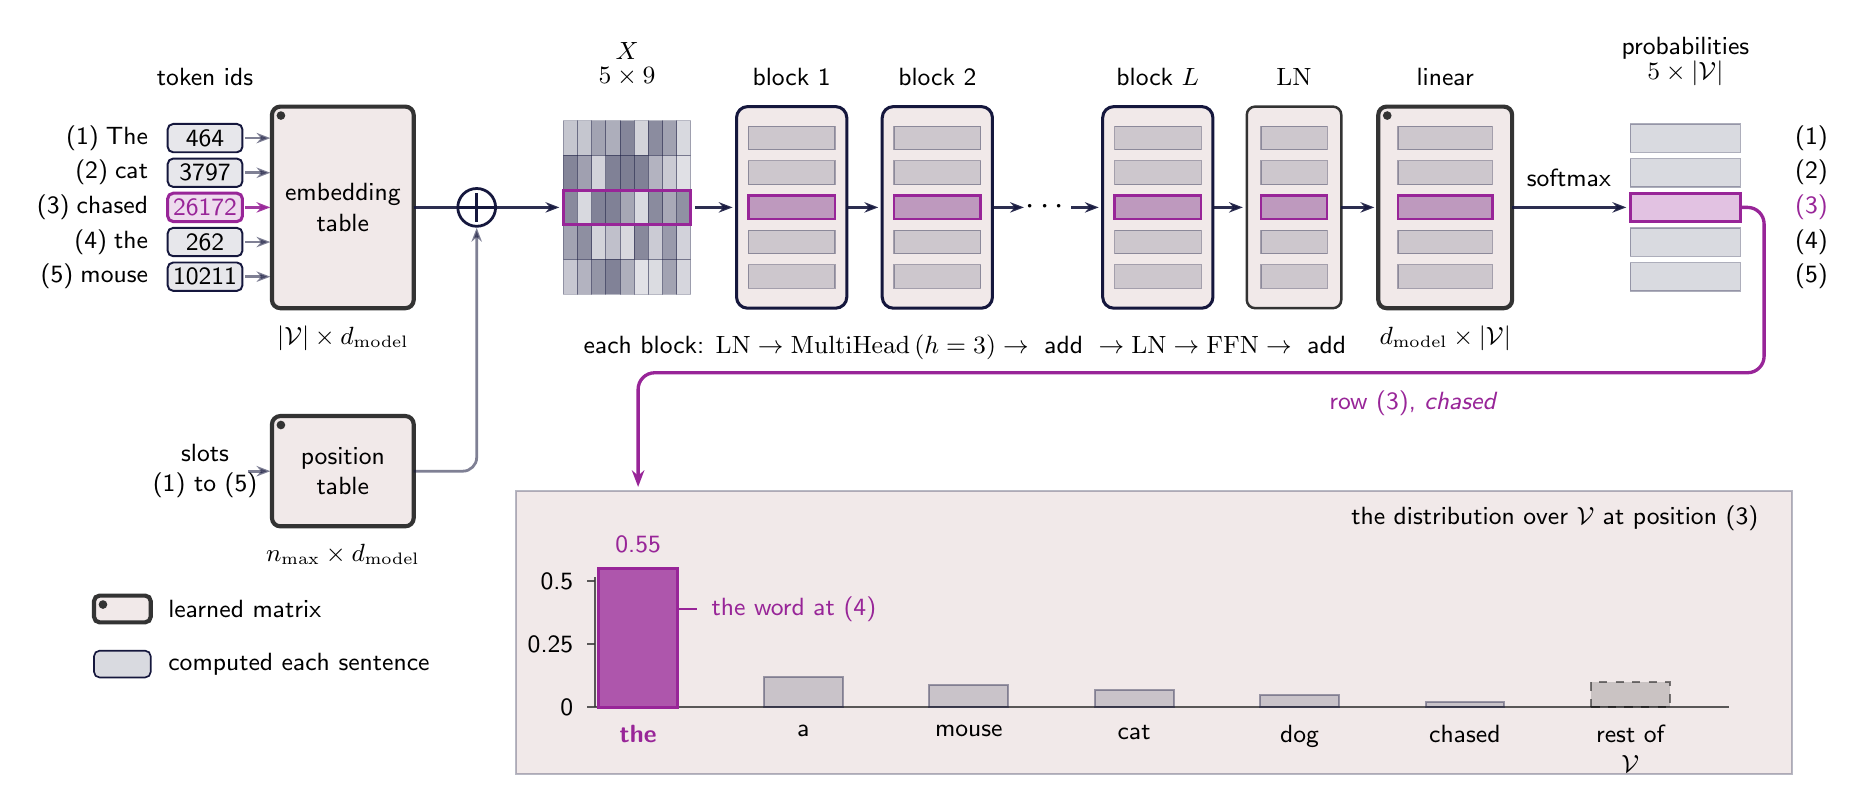
\begin{tikzpicture}[
    every node/.style={font=\sffamily},
]

\definecolor{c1}{HTML}{15173D}
\definecolor{c2}{HTML}{982598}
\definecolor{c3}{HTML}{E491C9}
\definecolor{c4}{HTML}{F1E9E9}
\definecolor{axiscolor}{HTML}{333333}
\definecolor{labelcolor}{HTML}{000000}
\definecolor{greenok}{HTML}{4CAF50}

% ================================================================
% GEOMETRY, fixed before any TikZ was written.
%
% The stream runs left to right along y = 3.0, which is row (3),
% chased. Five positions are rows at y = 3.0 + {0.88, 0.44, 0, -0.44,
% -0.88}: (1) on top, (5) at the bottom. Every full-height box is
% y in [1.72, 4.28], so the whole chain lines up.
%
%   x  1.18-2.13  token id boxes         (words right-anchored at 1.05)
%   x  2.50-4.30  embedding table        (learned: thick outline + dot)
%   x  4.30-6.15  stream segment, plus circle centred at 5.10
%   x  2.50-4.30  position table, y in [-1.05, 0.35], branch into the plus
%   x  6.20-7.82  X grid, 5 x 9 cells of 0.18 x 0.44
%   x  8.40-9.80  block 1    10.25-11.65 block 2    13.05-14.45 block L
%                 ellipsis at 12.35
%   x 14.88-16.08 LN (grey, no dot)      16.55-18.25 linear (learned)
%   x 19.75-21.15 probabilities column, position labels at 21.25
%
% THE c2 THREAD, unbroken. Row (3) is highlighted in the id column, in
% X, inside every block, inside LN, inside the linear map, and in the
% probability column, then leaves the column rightwards at y = 3.0, runs
% down to y = 0.9, left to x = 7.15 and down into the chart panel,
% landing directly above the tallest bar. LN and the linear map carry
% the same five-row interior as the blocks so the trace never stops;
% their names sit on the header line at y = 4.42 with the others.
%
% Chart panel x in [5.60, 21.80], y in [-4.20, -0.60].
%   baseline y = -3.35, 3.2 cm per unit of probability,
%   axis at x = 6.60, bars of width 1.0 at x = 7.15 + k*2.10, k = 0..6.
%
% Legend fills the lower left, x in [0.3, 5.2], clear of the panel.
% Bounding box roughly x in [-0.9, 21.8], y in [-4.2, 4.9]: wide.
% ================================================================

\def\sy{3.0}        % stream: row (3)
\def\rp{0.44}       % row pitch
\def\base{-3.35}    % chart baseline
\def\sc{3.2}        % chart: cm per unit of probability

\tikzset{
  learn/.style={
    draw=axiscolor, line width=1.5pt, fill=c4, text opacity=1,
    rounded corners=3pt, align=center,
    font=\sffamily\small, text=black,
  },
  norm/.style={
    draw=axiscolor, line width=0.9pt, fill=c4, text opacity=1,
    rounded corners=3pt, align=center,
    font=\sffamily\small, text=black,
  },
  blk/.style={
    draw=c1, line width=1.1pt, fill=c4, rounded corners=4pt,
    minimum width=1.4cm, minimum height=2.56cm, inner sep=0pt,
  },
  arr/.style={-{Stealth[length=5pt]}, line width=1.1pt, c1, opacity=0.9},
  branch/.style={-{Stealth[length=5pt]}, line width=1.0pt, c1,
                 opacity=0.55, rounded corners=5pt},
  hd/.style={font=\sffamily\small, text=black, anchor=south},
  shp/.style={font=\sffamily\small, text=black, anchor=north},
  op/.style={font=\sffamily\small, text=black},
  lab/.style={font=\sffamily\small, text=black},
  note/.style={font=\sffamily\small, text=c2},
}

\newcommand{\dotmark}[1]{\fill[axiscolor] ($(#1.north west)+(0.14,-0.14)$)
    circle (0.055);}
% row y for position \p (1..5)
\newcommand{\ry}[1]{\sy+(3-#1)*\rp}

% five token rows inside a box: #1 centre x, #2 half width.
% row (3) is c2; this is the thread and it must appear in every box on
% the stream, including LN and the linear map.
\newcommand{\rowstack}[2]{%
  \foreach \p in {1,...,5} {
    \pgfmathsetmacro{\y}{\ry{\p}}
    \fill[c1, opacity=0.16] (#1-#2, \y-0.15) rectangle ++({2*#2}, 0.30);
    \draw[c1, opacity=0.35, line width=0.4pt]
        (#1-#2, \y-0.15) rectangle ++({2*#2}, 0.30);
  }
  \fill[c2, opacity=0.28] (#1-#2, \sy-0.15) rectangle ++({2*#2}, 0.30);
  \draw[c2, line width=0.9pt] (#1-#2, \sy-0.15) rectangle ++({2*#2}, 0.30);
}

% the residual add: the stream line is the horizontal bar of the plus.
% white disc, c1 rim, then the line re-stroked across it, then the
% vertical stroke. Never a text glyph.
\newcommand{\plusnode}[2]{%
  \fill[white] (#1, #2) circle (0.24);
  \draw[c1, line width=1.0pt] (#1, #2) circle (0.24);
  \draw[c1, line width=1.1pt] (#1-0.24, #2) -- (#1+0.24, #2);
  \draw[c1, line width=1.1pt] (#1, #2-0.18) -- (#1, #2+0.18);
}

\pgfmathsetseed{2718}

% ================================================================
% (1) token ids
% ================================================================
\node[hd] at (1.65, 4.42) {token ids};

\foreach \p/\w in {1/The, 2/cat, 3/chased, 4/the, 5/mouse} {
    \pgfmathsetmacro{\y}{\ry{\p}}
    \node[font=\sffamily\small, anchor=east] at (1.05, \y)
        {\textcolor{black}{(\p)}\;\textcolor{black}{\w}};
}
\foreach \p/\id in {1/464, 2/3797, 4/262, 5/10211} {
    \pgfmathsetmacro{\y}{\ry{\p}}
    \node[draw=c1, line width=0.7pt, fill=c1, fill opacity=0.10,
          text opacity=1, rounded corners=2pt, minimum width=0.95cm,
          minimum height=0.36cm, inner sep=0pt,
          font=\sffamily\small, text=black] at (1.65, \y) {\id};
}
\node[draw=c2, line width=1.1pt, fill=c2, fill opacity=0.16,
      text opacity=1, rounded corners=2pt, minimum width=0.95cm,
      minimum height=0.36cm, inner sep=0pt,
      font=\sffamily\small, text=c2] at (1.65, \sy) {26172};

% ================================================================
% (2) embedding table and position table
% ================================================================
\node[learn, minimum width=1.8cm, minimum height=2.56cm] (emb)
    at (3.4, \sy) {embedding\\table};
\dotmark{emb}
\node[shp] at (3.4, 1.62) {$\lvert\mathcal{V}\rvert \times d_{\mathrm{model}}$};

\node[learn, minimum width=1.8cm, minimum height=1.40cm] (pos)
    at (3.4, -0.35) {position\\table};
\dotmark{pos}
\node[shp] at (3.4, -1.15) {$n_{\max} \times d_{\mathrm{model}}$};

\node[lab, align=center] at (1.65, -0.35) {slots\\(1) to (5)};
\draw[branch] (2.20, -0.35) -- (2.48, -0.35);

\foreach \p in {1,2,4,5} {
    \pgfmathsetmacro{\y}{\ry{\p}}
    \draw[branch] (2.16, \y) -- (2.48, \y);
}
\draw[-{Stealth[length=5pt]}, line width=1.0pt, c2, opacity=0.9]
    (2.16, \sy) -- (2.48, \sy);

% ---------------------------------------------------------------- stream
\draw[arr] (4.30, \sy) -- (6.15, \sy);
\draw[branch] (4.30, -0.35) -- (5.10, -0.35) -- (5.10, 2.74);
\plusnode{5.10}{\sy}

% ================================================================
% (3) X
% ================================================================
\node[hd] at (7.01, 4.76) {$X$};
\node[hd, text=black] at (7.01, 4.42) {$5 \times 9$};
\foreach \p in {1,...,5} {
    \pgfmathsetmacro{\y}{\ry{\p}}
    \foreach \c in {0,...,8} {
        \pgfmathsetmacro{\op}{0.12+0.45*rnd}
        \fill[c1, opacity=\op] (6.2+\c*0.18, \y-0.22) rectangle ++(0.18, 0.44);
        \draw[c1, opacity=0.30, line width=0.3pt]
            (6.2+\c*0.18, \y-0.22) rectangle ++(0.18, 0.44);
    }
}
\draw[c2, line width=1.1pt] (6.2, \sy-0.22) rectangle (7.82, \sy+0.22);

% ================================================================
% (4) the stack of L blocks
% ================================================================
\foreach \cx/\name in {9.1/{block 1}, 10.95/{block 2}, 13.75/{block $L$}} {
    \node[blk] at (\cx, \sy) {};
    \node[hd] at (\cx, 4.42) {\name};
    \rowstack{\cx}{0.55}
}
\draw[arr] (7.87, \sy) -- (8.35, \sy);
\draw[arr] (9.80, \sy) -- (10.20, \sy);
\draw[arr] (11.65, \sy) -- (12.05, \sy);
\draw[arr] (12.65, \sy) -- (13.00, \sy);
\node[font=\sffamily\large, text=black] at (12.35, \sy) {$\cdots$};

\node[lab, anchor=north, align=center] at (11.3, 1.50)
    {each block: $\mathrm{LN} \to \mathrm{MultiHead}\,(h = 3) \to{}$ add
     ${}\to \mathrm{LN} \to \mathrm{FFN} \to{}$ add};

% ================================================================
% (5) output head
% ================================================================
% LN: a neutral grey box, deliberately without the learned-matrix dot.
\node[norm, minimum width=1.2cm, minimum height=2.56cm] (ln)
    at (15.48, \sy) {};
\rowstack{15.48}{0.42}
\node[hd] at (15.48, 4.42) {$\mathrm{LN}$};
\draw[arr] (14.45, \sy) -- (14.83, \sy);

\node[learn, minimum width=1.7cm, minimum height=2.56cm] (lin)
    at (17.40, \sy) {};
\dotmark{lin}
\rowstack{17.40}{0.60}
\node[hd] at (17.40, 4.42) {linear};
\node[shp] at (17.40, 1.62) {$d_{\mathrm{model}} \times \lvert\mathcal{V}\rvert$};
\draw[arr] (16.08, \sy) -- (16.50, \sy);

\draw[arr] (18.25, \sy) -- (19.70, \sy);
\node[op, anchor=south] at (18.97, \sy+0.14) {softmax};

% probabilities column
\node[hd] at (20.45, 4.76) {probabilities};
\node[hd, text=black] at (20.45, 4.42) {$5 \times \lvert\mathcal{V}\rvert$};
\foreach \p in {1,2,4,5} {
    \pgfmathsetmacro{\y}{\ry{\p}}
    \fill[c1, opacity=0.16] (19.75, \y-0.18) rectangle ++(1.4, 0.36);
    \draw[c1, opacity=0.35, line width=0.5pt]
        (19.75, \y-0.18) rectangle ++(1.4, 0.36);
    \node[lab, anchor=west] at (21.72, \y) {(\p)};
}
\fill[c2, opacity=0.28] (19.75, \sy-0.18) rectangle ++(1.4, 0.36);
\draw[c2, line width=1.0pt] (19.75, \sy-0.18) rectangle ++(1.4, 0.36);
\node[note, anchor=west] at (21.72, \sy) {(3)};

% ================================================================
% (6) the thread from row (3) down into the chart
% ================================================================
\draw[-{Stealth[length=6pt]}, line width=1.2pt, c2, rounded corners=6pt]
    (21.15, \sy) -- (21.45, \sy) -- (21.45, 0.90) -- (7.15, 0.90) -- (7.15, -0.55);
\node[note, anchor=north] at (17.0, 0.80) {row (3), \emph{chased}};

% ================================================================
% (7) the distribution at position (3)
% ================================================================
\fill[c4] (5.60, -4.20) rectangle (21.80, -0.60);
\draw[c1, opacity=0.30, line width=0.7pt] (5.60, -4.20) rectangle (21.80, -0.60);
\node[font=\sffamily\small, text=black, anchor=east] at (21.50, -0.95)
    {the distribution over $\mathcal{V}$ at position (3)};

% axis
\draw[axiscolor, opacity=0.8, line width=0.7pt] (6.60, \base) -- (6.60, -1.70);
\draw[axiscolor, opacity=0.8, line width=0.7pt] (6.60, \base) -- (21.00, \base);
\foreach \v in {0, 0.25, 0.5} {
    \pgfmathsetmacro{\y}{\base+\v*\sc}
    \draw[axiscolor, opacity=0.8, line width=0.7pt] (6.60, \y) -- (6.50, \y);
    \node[lab, anchor=east] at (6.45, \y) {\v};
}

\foreach \k/\w/\v in {0/the/0.55, 1/a/0.12, 2/mouse/0.09, 3/cat/0.07,
                      4/dog/0.05, 5/chased/0.02} {
    \pgfmathsetmacro{\x}{7.15+\k*2.10}
    \pgfmathsetmacro{\h}{\v*\sc}
    \ifnum\k=0
        \fill[c2, opacity=0.75] (\x-0.5, \base) rectangle ++(1.0, \h);
        \draw[c2, line width=1.0pt] (\x-0.5, \base) rectangle ++(1.0, \h);
        \node[font=\sffamily\small\bfseries, text=c2, anchor=north]
            at (\x, \base-0.10) {\w};
    \else
        \fill[c1, opacity=0.18] (\x-0.5, \base) rectangle ++(1.0, \h);
        \draw[c1, opacity=0.40, line width=0.7pt]
            (\x-0.5, \base) rectangle ++(1.0, \h);
        \node[font=\sffamily\small, text=black, anchor=north]
            at (\x, \base-0.10) {\w};
    \fi
}
% the rest of the vocabulary, lumped
\pgfmathsetmacro{\xr}{7.15+6*2.10}
\fill[labelcolor, opacity=0.16] (\xr-0.5, \base) rectangle ++(1.0, {0.10*\sc});
\draw[labelcolor, opacity=0.5, line width=0.7pt, dashed]
    (\xr-0.5, \base) rectangle ++(1.0, {0.10*\sc});
\node[font=\sffamily\small, text=black, anchor=north, align=center]
    at (\xr, \base-0.10) {rest of\\$\mathcal{V}$};

\node[font=\sffamily\small, text=c2, anchor=south] at (7.15, {\base+0.55*\sc+0.08})
    {0.55};
\draw[c2, line width=0.7pt] (7.65, -2.10) -- (7.90, -2.10);
\node[note, anchor=west] at (7.96, -2.10) {the word at (4)};

% ================================================================
% (8) legend
% ================================================================
\node[draw=axiscolor, line width=1.5pt, fill=c4, rounded corners=2pt,
      minimum width=0.72cm, minimum height=0.34cm, inner sep=0pt] (lgA)
    at (0.60, -2.10) {};
\dotmark{lgA}
\node[lab, anchor=west] at (1.06, -2.10) {learned matrix};

\node[draw=c1, line width=0.6pt, fill=c1, fill opacity=0.16,
      rounded corners=2pt, minimum width=0.72cm, minimum height=0.34cm,
      inner sep=0pt] at (0.60, -2.80) {};
\node[lab, anchor=west] at (1.06, -2.80) {computed each sentence};

\end{tikzpicture}
\end{document}
